\section{Procedura operativa}

	Si è acceso il tetrodo regolando la tensione del catodo $U_F$ = \SI{8.0 \pm 0.1}{\volt}
	in modo da innescare l'emissione di $e^{-}$ per effetto termoionico.

	In una prima fase si è regolata la tensione sulla griglia d'anodo imponendo $U_A=$ \SI{70 \pm 0.1}{\volt},	dopodichè si è modificata la tensione $U_G$ sulla griglia di controllo aumentandola fino alla comparsa di tre bande luminose arancioni.
	La griglia di controllo ha una duplice funzione:
	\begin{itemize}
	\item  stabilire un campo elettrico sulla superficie del catodo favorendo l'emissione di elettroni e aumentando di fatti la luminosità  delle bande;
	\item trattandosi di una fitta rete di fili sottili permette il passaggio degli elettroni e fissandone il potenziale permette di generare un campo uniforme fino alla griglia d'anodo (come in un condensatore a facce piane e parallele); al diminuire della tensione $U_G$ si nota infatti un cambiamento nella forma delle bande luminose (si distorcono ai bordi) venendo a mancare l'uniformità  del campo.
	\end{itemize}

	Gli elettroni risultano accelerati dalla d.d.p. $U_A-U_G$.

\paragraph{}
	Si è osservato che aumentando la tensione $U_A$ partendo da $\SI{0}{\volt}$ si ottiene
	dapprima la comparsa di una banda luminosa nella zona della griglia d'anodo, quindi lo spostamento della riga verso il catodo e successivamente, continuando ad aumentare  la tensione, la comparsa di un'altra banda sull'anodo, che evolve come la precedente.
	 Nel range di tensioni permesse dall'apparato è possibile vedere contemporaneamente 3 bande.

		Questo andamento è da imputarsi al fatto che il trasferimento
		di energia negli urti tra $e^{-}$ e atomi di Ne sia
		quantizzato: un urto anelastico è possibile esclusivamente quando hanno gli elettroni hanno energia maggiore o uguale
		al gap energetico tra primi livelli eccitati liberi.

		Poichè l'energia degli $e^{-}$ è proporzionale alla distanza
		percorsa dalla griglia di controllo ed alla d.d.p. $U_A-U_G$,
		all'aumentare di $U_A$ si riduce
		la distanza necessaria affinchè gli $e^-$ abbiano l'energia sufficiente
		ad eccitare gli atomi di Ne, pertanto la banda si sposta verso il catodo.

		All'ulteriore aumento del campo accelerante dopo il
		primo urto, e conseguentemente all'eccitazione degli
		atomi di neon, gli elettroni acquisiscono un energia
		sufficiente per rieccitare gli atomi
		di neon in un tratto successivo del tetrodo ;
		a ciò corrisponde la comparsa delle ulteriori righe colorate.
\paragraph{}
	Si è proceduto alla misura della d.d.p. $U_A-U_G$ di apparizione delle bande luminose. Ogni membro del gruppo ha ripetuto la misura, il risultato della media è di seguito riportato:

	\begin{table}[H]
 		\centering
		\begin{tabular}{cc}
 			\toprule
 			$\#$  &  $U_A- U_G$\\
  			\midrule
  			$1$ & \SI{15.6 \pm 1.0}{\volt}\\
  			$2$ &  \SI{32.1 \pm 1.0}{\volt}\\
  			$3$ & \SI{53.5 \pm 1.0}{\volt}\\
  			\bottomrule
 		\end{tabular}
	\label{tab:a}
	\end{table}



	Ci si aspetta, almeno in prima approssimazione, che le differenze fra le d.d.p $U_A-U_G$ tra due bande successive sia la differenza di energia tra i primi livelli eccitati liberi degli atomi di Neon.
	In particolare si ottiene $\Delta_{12} = \SI{16.5 \pm 1.4}{\volt}$ e $\Delta_{23} = \SI{21.4 \pm 1.4}{\volt}$, che sono da confrontarsi con la differenze di energia dei primi livelli eccitati del Neon rispetto al fondamentale ($1s^2 2s^2 2p^6$):
	$$E_1 \simeq \SI{16.7}{\volt} \quad (1s^2 2s^2 2p^5 3s) \qquad \text{ e } \qquad E_2 \simeq \SI{18.6}{\volt} \quad (1s^2 2s^2 2p^5 3p).$$

\bigskip
	Si è settato apparato strumentale in modo che
	la tensione $U_A$ sia in modalità  ramp: varierà  automaticamente tra $\SI{0}{\volt}$ e il massimo permesso dall'apparato (\SI{80.0 \pm 0.5}{\volt}). La tensione della griglia di controllo è invece lasciata fissa al valore $U_G = \SI{4.0 \pm 0.1}{\volt}$.

Il collettore è collegato al generatore di tensione mediante un amplificatore a transimpedenza
	che fornisce in uscita un segnale in tensione proporzionale alla corrente di collettore $I_C$.

	Attraverso la modalità  X-Y dell'oscilloscopio si è quindi
	osservato l'andamento della curva $I_C \text{ vs } U_A$ al
	variare di $U_E$.

	L'applicazione di una d.d.p tra griglia d'anodo e collettore ha lo scopo di creare un campo elettrico frenante per gli elettroni che emergono dall'anodo verso il collettore.

	In \figurename{ \ref{fig:ue}} sono riportati gli andamenti osservati.

\begin{figure}[h!]
		\centering
		 \subfloat[$U_E=\SI{1.0 \pm 0.1}{\volt}$]{
		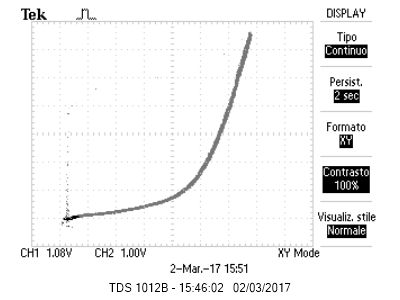
\includegraphics[scale=0.6]{../Figs-tabs/ue3.png}
		\label{f:ue1}
		}
		 \subfloat[$U_E= \SI{3.4 \pm 0.1}{\volt}$]{
		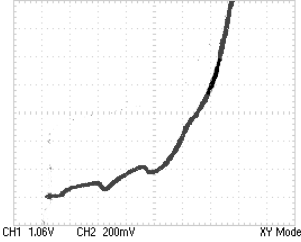
\includegraphics[scale=0.6]{../Figs-tabs/ue34.png}
		\label{f:ue3.4}
		}
		 \subfloat[$U_E= \SI{7.5 \pm 0.6}{\volt}$]{
		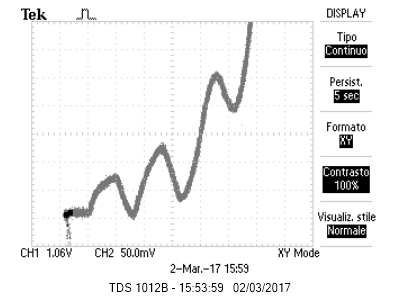
\includegraphics[scale=0.6]{../Figs-tabs/ue75.png}
		\label{f:ue7.5}
		}
		\caption{$I_C$ vs $U_A$ al variare di $U_E$ in modalità X-Y}
	\label{fig:ue}
\end{figure}
	Come è possibile osservare da \figurename{ \ref{f:ue1}} e \figurename{ \ref{f:ue3.4}}
	per valori bassi del campo decelerante $U_E$ la quasi totalità  degli $e^{-}$, anche qualora facciano
	urti anelastici, raggiunge il collettore.
	Aumentando $U_E$ si osserva un decremento
	di $I_C$, ciò risulta compatibile col fatto che gli $e^{-}$
	dopo aver ceduto energia per eccitare gli atomi di Ne
	non hanno energia sufficiente a superare il campo di decelerazione.

In \figurename{ \ref{f:ue7.5}} è evidente il classico andamento  : all'aumentare di $U_A$ corrisponde un aumento di $I_C$ fino ad un massimo, che coincide col momento in cui gli $e^-$ iniziano ad avere energia sufficiente per eccitare gli atomi di Neon, a questo evento corrisponde la comparsa della prima banda.
	Il minimo che segue è nel punto in cui la banda si stacca dalla griglia d'anodo: in questo caso la maggior parte degli elettroni supera la griglia con energia quasi nulla: vengono fermati dal campo frenante, non arrivando quindi sul collettore.
	All'aumentare della tensione $U_A$ la corrente torna ad aumentare fino a quando gli elettroni non avranno nuovamente l'energia necessaria ad eccitare il neon.

	Dalla regolazione di $U_E$ si sono settati i minimi della curva
	$I_C \text{ vs } U_A$ in corrispondenza dello zero.
	Si è regolato il valore di $U_A$ in maniera da osservare il maggior
	numero di massimi osservabili sullo schermo dell'oscilloscopio,
	è stato inoltre necessario regolare il guadagno dell'amplificatore
	in maniera da non saturare l'OpAmp.

	A seguito si sono acquisite le due tracce di $U_A$ e $\propto I_C$ al variare di
	$U_E$ da $\SI{9}{\volt}$ a $\SI{0}{\volt}$. Per  tali acquisizioni, qualora non si siano
	verificati problemi a rilevare i picchi, sono state
	osservate le $U_A$ corrispondenti ai massimi di $I_C$.

\sisetup{table-figures-decimal = 1, table-figures-exponent = 0, table-figures-integer = 2, table-figures-uncertainty = 1}

	\begin{table}[H]
		\centering
		\begin{tabular}{SSSSS}
			\toprule
			{\multirow{2}{*}{$U_E\;[\si{\volt}]$}}  &  \multicolumn{4}{c}{$U_A-U_G\;[\si{\volt}]$}\\
			 &	{1} & {2} & {3} & {4}\\
			\midrule
			9.6(1) & 15.2(8) & 33.4(8) & 53.3(8) & 73.2(8)\\
			9.0(1) & 15.6(8) & 32.5(8) & 52.9(8) & 73.2(8)\\
			8.0(1) & 14.3(8) & 32.5(8) & 52.5(8) & 72.8(8)\\
			6.9(1) & 15.2(8) & 32.5(8) & 53.3(8) &\\
			6.0(1) & 14.7(8) & 32.1(8) & &\\
			5.0(1) & 13.5(8) & 31.7(8) & &\\
			4.0(1) & 12.6(8) & & &\\
			3.0(1) & 13.0(8) & & &\\
			\bottomrule
		\end{tabular}
		\label{tab:a}
	\end{table}
Le caselle vuote corrispondo a massimi non misurabili.

Si è poi proceduto ad un fit lineare, ottenendo i seguenti risultati:
	\begin{table}[H]
		\centering
		\begin{tabular}{ccc}
			$\Delta V_1 = \SI{14.3 \pm 0.3}{\volt}$ && $\chi^2/ndof = 13/7$\\
			$\Delta V_2 = \SI{32.5 \pm 0.3}{\volt}$ && $\chi^2/ndof = 2.5/5$\\
			$\Delta V_3 = \SI{53.0 \pm 0.4}{\volt}$ && $\chi^2/ndof = 0.8/3$\\
			$\Delta V_4 = \SI{73.1 \pm 0.5}{\volt}$ && $\chi^2/ndof = 0.2/2$\\
		\end{tabular}
	\end{table}
	Si riporta il fit in \figurename{ \ref{fit}}.

		\begin{figure} [!h]
			\centering
			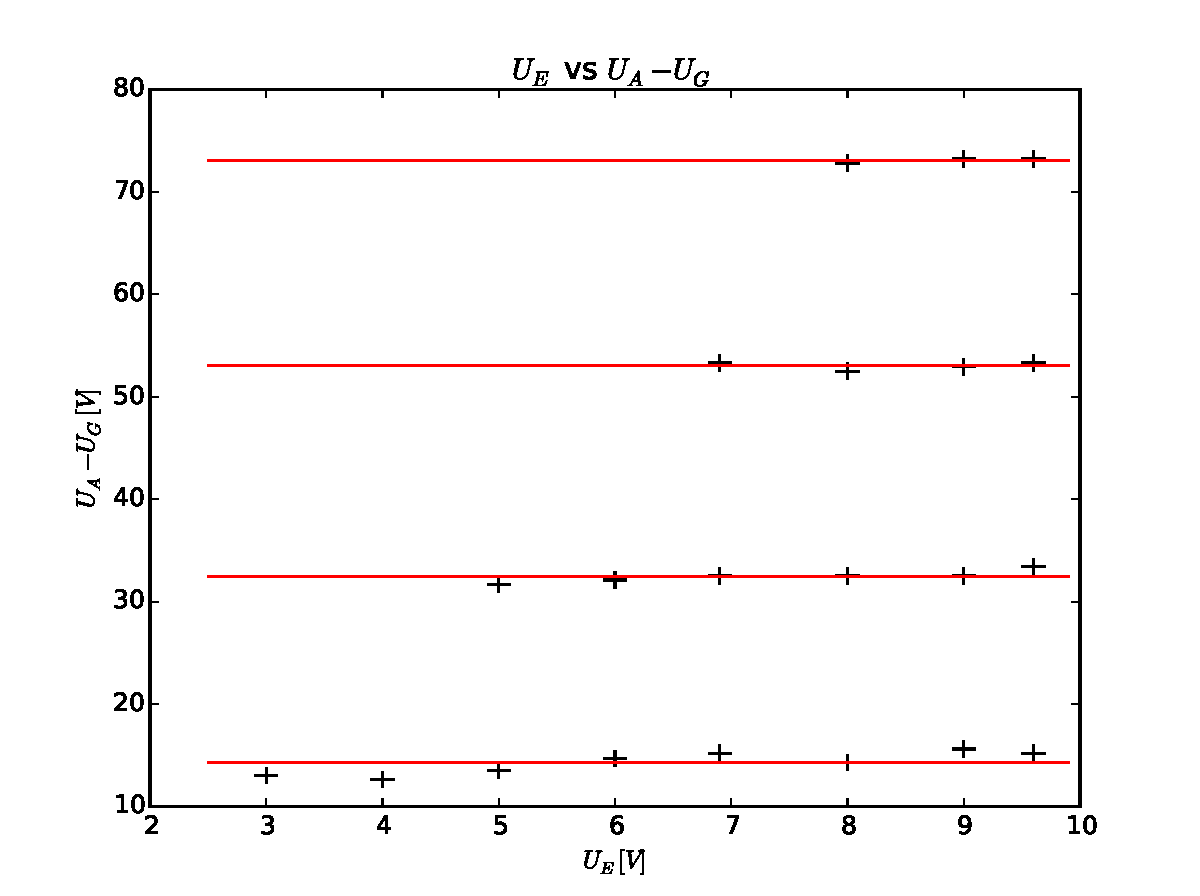
\includegraphics[width=0.9\textwidth]{../Figs-tabs/fit.pdf}
			\caption{Dati raccolti e fit.}
			\label{fit}
		\end{figure}

	Le differenze tra i massimi sono dunque:
	$$\Delta_{12}=\SI{18.2\pm 0.4}{\volt} \qquad \Delta{23}=\SI{20.5 \pm 0.5}{\volt} \qquad \Delta{34}=\SI{20.1 \pm 0.6}{\volt}$$
	Si osserva che questi risultati sono in accordo con quelli trovati alla verifica qualitativa della comparsa delle frange.

\subsection{Note}
Nell'acquisizione dei massimi di $I_C$ contro $U_A$ si è preso come errore
l'incertezza stessa del dato identificato come valore massimo, poiché essa è confrontabile con
la larghezza della regione (pressoché piatta) del massimo e pertanto non riteniamo
di poter sfruttare il numero di dati raccolti per ridurre l'errore in modo sighificativo.

Si sono propagati gli errori sistematici (risultanti da differenze rispetto a valori fissi
o simili operazioni) separatamente rispetto a quelli statistici; in particolare
nell'eseguire i fit si è considerato solo questi ultimi.

\section{Conclusioni}

